%\chapter{\normalsize{BACKGROUND OF SATELLITE REMOTE SENSING}}
\chapter{\normalsize{BASIC PRINCIPLES OF SATELLITE REMOTE SENSING}}
\section{Definition}
\paragraph{}
\textbf{Remote sensing} is the science (and to some extent, art) of acquiring information about the Earth's surface without actually being in contact with it. This is done by sensing and recording reflected or emitted energy and processing, analysing, and applying that information.
\paragraph{}
In much of remote sensing, the process involves an interaction between incident radiation 
and the targets of interest. This is exemplified by the use of imaging systems where the 
following seven steps are involved. However that remote sensing also involves the 
sensing of emitted energy and the use of non-imaging sensors. 

\begin{figure}[H]
\begin{center}
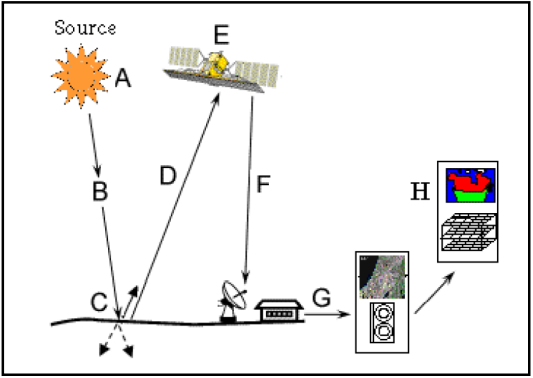
\includegraphics[scale=0.8]{image0.png} %\cite{umhe}
\end{center}
\caption{Remote sensing process}
\label{Remote sensing process}%\cite{ABIA}
\end{figure}
\begin{description}
\item[Step 1-Energy Source or Illumination (A)] : the first requirement for remote sensing is to have  an energy source which illuminates or  provides electromagnetic energy to the target of interest.
\item[Step 2-Radiation and the Atmosphere (B)]: as the energy travels from its source to the target, it will come in contact with and interact with the atmosphere it passes through. This interaction may take place a second time as  the energy travels from the target to the sensor. 
\item[Step 3-Interaction with the Target (C)] : once the energy makes its way to the target through the atmosphere, it interacts with the target depending on the properties of both the target and the radiation.
\item[Step 4-Recording of Energy by the Sensor (D)] : after the energy has been scattered by, or emitted from the target, we require a sensor (remote - not in contact with the target) to collect and record the electromagnetic radiation. 
\item[Step 5-Transmission, Reception, and Processing (E)]: the energy recorded by the sensor has to be transmitted, often in electronic form, to a receiving and processing station where the data are processed into an image (hardcopy and/or digital).
\item[Step 6-Interpretation and Analysis (F)] the processed image is interpreted, visually and/or  digitally or electronically, to extract information about the target which was illuminated. 
\item[Step 7-Application (G) ] the final element of the remote sensing process is achieved when we  apply the information we have been able to extract from the imagery about the target in order  to better understand it, reveal some new information, or assist in solving a particular problem. 
\end{description}
%\section{Présentation du lieu du stage}
\section{Electromagnetic Spectrum}
\paragraph{}
Solar radiation can be divided into different wavelengths call Electromagnetic spectrum as depicted by the figure below.
\begin{figure}[H]
\begin{center}
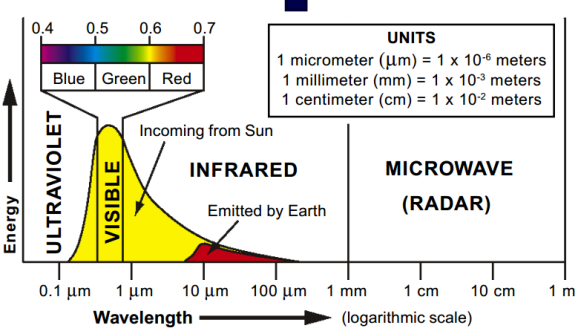
\includegraphics[scale=0.8]{image1.png} %\cite{umhe}
\end{center}
\caption{Electromagnetic spectrum}
\label{Electromagnetic spectrum}%\cite{ABIA}
\end{figure}
\paragraph{}
Most Multispectral satellite can acquire data in visible and infrared region (including the thermal infrared region).  Nowdays there is an increasing demand for data in microwaves region, because the microwave energy can penetrate through the cloud.
\section{Source of radiation}
\paragraph{}
We have two major source of radiation: the sun and the earth. \newline
The \textbf{sun} is the mayor source of radiation with highest energy in visible, near infrared and short-wave infrared region.\newline
The \textbf{earth surface} can also emit energy usually in thermal Infrared and microwaves region.
\section{Interaction in the atmosphere}
\begin{wrapfigure}{I}{0.5\textwidth}
%\begin{figure}[H]
\begin{center}
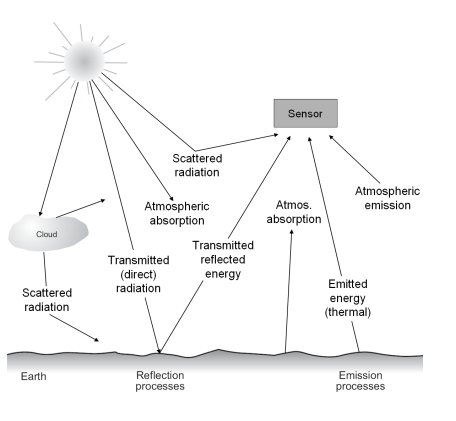
\includegraphics[scale=0.8]{image3.png} %\cite{umhe}
\end{center}
\caption{radiance at the sensor}
\label{radiance at the sensor}%\cite{ABIA}
%\end{figure}
\end{wrapfigure}
\paragraph{}
Before radiation used for remote sensing reaches the Earth's surface it has to travel through some distance of the Earth's atmosphere. Different processes occur due to the presence of particles and gases in the atmosphere. Some get \textbf{scattered}, some get \textbf{absorbed}, some managed to transmit through the atmosphere and get \textbf{absorbed}  by the earth, and some get \textbf{reflected} . This reflected energy is captured by the sensor on board a satellite.
The earth equally emits energy, the amount of energy emitted is directly proportional to the heat level of the part of the earth that emit it. This emitted energy can also be recorded by sensors on board a satellite if that sensor has capabilities to record energy in thermal infrared region. A sensor on board a satellite can record \textbf{re-mitted}  or \textbf{reflected} radiation depending on the capabilities of the sensors.













   